\subsubsection{Randomised Strat ME}

\paragraph{Outline}
Closest thing we have to an INSS WR template. 1) Find super-efficient the bonuses. 2) Pick having those in mind, whether that is picking them, or countering them).
\url{https://www.youtube.com/watch?v=8rpfNJT8JPc}

3x4, neutrals 2/4, wastelands 7/10, base +5

\paragraph{Map Dynamics}

Follow Strat ME's Map Dynamics section.

\paragraph{Picking Logic}

The idea in Randomized Strat ME, is that every bonus value is anything in the range of [-1,+1]. So for example Scandinavia in Strat ME is a +3 bonus, here it can be either a +2, or a +3 or a +4 bonus. While this introduces some variance from game to game, it can potentially create one-sided distributions. Though I would put as an asterisk here and for most templates, that a distribution is one-sided only if both players find the best picks and moves assuming also that the above set is truly one-sided. 
\\
\\For example \href{https://www.warzone.com/MultiPlayer?GameID=41209813}{here}, you can see the similarities in our sets. There are 6 super efficient bonuses on the map and you cannot really deviate from picking those. I chose to combo 3 and 6 this way precisely in case we mirror all 6 of our picks to get a safe WR on my 3rd covered by my 6th. My comment/comparison of this (and other templates) to INSS, is sort of figurative. In INSS there are usually forced picks and lines, making it literally impossible to make a comeback (assuming your opponent won't misplay). In this template, despite the variance WR and RMO introduce, you should be able to win in picks.
\\
\\
Super-efficient +6 bonuses are the hardest to evaluate (6 territories for +6 income). For example, you can gamble everything in finishing it by T2 like \href{https://www.warzone.com/MultiPlayer?GameID=41386005}{here}, or approach it like \href{https://www.warzone.com/MultiPlayer?GameID=41513105}{7ate9 vs Aika} and \href{https://www.warzone.com/MultiPlayer?GameID=41137719}{7ate9 vs neet}. Part of what makes them strong is they can surprise your opponent, especially if you don't get eliminated in another region.
\\
\\
I'll list some example games of different bonuses and how they have been picked and you can judge yourself if the approach is correct or not.
\begin{itemize}
    \item Canada: If it's 7 for +5 or +4 it's only good as a counter pick on your 6th really like \href{https://www.warzone.com/MultiPlayer?GameID=38731303}{here} in LND's picks, albeit he never got it, or \href{https://www.warzone.com/MultiPlayer?GameID=25588607}{in mod's picks}. If it's 7 for +6, there's space to experiment. 
    \begin{itemize}
        \item \href{https://www.warzone.com/MultiPlayer?GameID=22899460}{For example here}, Rufus picks in an unconventional way of expecting a split of 1/2 and striving for a cover pick in Africa, a safe bonus in Asia and Canada that can come off unexpected. I suspect the idea to be to counter the expansion of the opponent that gets WR+CA+SA or a similar set. But Octane reached the double border T2 with a 3attack, and then Rufus' 11 attackers only killed 6 defenders and Octane picked the right border. 
        \item In \href{https://www.warzone.com/MultiPlayer?GameID=26307050}{another example}, the distribution is messier. There are 4 super-efficient bonuses, out of which Australia is an extremely slow pick with 0 expansion. WAF and Ant sort of cover the same expansion regions, and WR has bad expansion (warlord in Scand. in awful position leading to useless leftovers, Caucasus +4). Beep goes for a set of 3/4 in NA. 
        \item A last \href{https://www.warzone.com/MultiPlayer?GameID=28054520}{example} of combo Canada/Greenland that's more of a puzzle of finding the winning idea without intel. It's WR, the opponent has awful expansion, the solution is stack all in towards that direction.
        \item "I found a surreal game after finishing this in \href{https://www.warzone.com/MultiPlayer?GameID=30043599}{Yelo vs malakkan} featuring quite possible the worst board I've ever seen, and a +6 in 3 turns from Quebec.
    \end{itemize}
    \item Greenland. 6 for 6 is very very good, but needs setup to get contact later in the game. 
    \begin{itemize}
        \item If opponent knows of it and sees you earlier with \href{https://www.warzone.com/MultiPlayer?GameID=41513105}{income/army advantage} say your prayers. If not gg wp
        \item Listing some example games like \href{https://www.warzone.com/MultiPlayer?GameID=38698474}{combo 1/3 Gree/Scandi}. Volatile set, extremely reliant on 1st pick Svalbard, worst case scenario it's 2/3/4 and you fight to get Greenland while holding the border. (2/3/6 is equivalent to a diceroll). \href{https://www.warzone.com/MultiPlayer?GameID=37060731}{Green/Canada combo}, where the game is decided on the leftovers left alive after T1. \href{https://www.warzone.com/MultiPlayer?GameID=31336179}{whatever this is} or \href{https://www.warzone.com/MultiPlayer?GameID=33030404}{whatever this is as well}.
    \end{itemize}
    \item West and East USA. As 7 for 6 they are quite decent, as long as the rest of the board is poor in income. (Though really like 990/1000 distributions it isn't worth it, and 9/10 it is it pairs to combo with CA like \href{https://www.warzone.com/MultiPlayer?GameID=30401282}{here} and \href{https://www.warzone.com/MultiPlayer?GameID=24344386}{here}).
    \item SA, Ant, WAf, EAf as good as they are in Strat ME. Antarctica has 57\% WR above 1800 rating as well as Eaf has 54.6\% WR. WAf and SA are slightly less valuable. WAf excels at having fast expansion within 2 turns to pretty much everything, but that's a potential downside here. If you overexpand and the opponent breaks Nigeria with a stack the game is lost.
    \item North Africa \& South Africa. Good in poor distributions and usually good later picks. For NAf \href{https://www.warzone.com/MultiPlayer?GameID=38078527}{NAf/Waf Combo}, \href{https://www.warzone.com/MultiPlayer?GameID=38399011}{NAf solo pick}, \href{https://www.warzone.com/MultiPlayer?GameID=33487996}{WAf FTB}. For SAf (rare) \href{https://www.warzone.com/MultiPlayer?GameID=32980493}{SAf/EAf Combo}, \href{https://www.warzone.com/MultiPlayer?GameID=30213538}{SAf/Ant Combo}, \href{https://www.warzone.com/MultiPlayer?GameID=26789968}{another SAf/Ant combo just because I can and that's really all that SA offers}, \href{https://www.warzone.com/MultiPlayer?GameID=28772609}{SAf/Ant/SA triple}.
    \item Middle East and Europe are 3 levels deep in Inception. For ME, only noteworthy ideas are at games like \href{https://www.warzone.com/MultiPlayer?GameID=22483437}{this}, where Rufus' idea on picks is to get 1/2/3 or 1/3/4 and eliminate on Svalbard/Greenland. (This concept is applicable in MME in games like \href{https://www.warzone.com/MultiPlayer?GameID=40135438}{this}, \href{https://www.warzone.com/MultiPlayer?GameID=35830458}{this} and even \href{https://www.warzone.com/MultiPlayer?GameID=40326611}{this}. Combo a bonus, then pick neighboring territories to force elimination.) Other applications in \href{https://www.warzone.com/MultiPlayer?GameID=24164262}{ME to combo with Caucasus}, \href{https://www.warzone.com/MultiPlayer?GameID=22563562}{ME/Caucasus/CR coverage through Iran}. The later sort of comes with how important Iran is in general in this map, due to its proximity to so many bonuses, like \href{https://www.warzone.com/MultiPlayer?GameID=25691500}{here}, as Iran can provide a counter to WR if needed. Europe, similarly, pairs for FTBs and combo with WR almost every time you'd consider picking it. Only distribution I found that's different pairs it with  \href{https://www.warzone.com/MultiPlayer?GameID=26984683}{Greenland/EU combo}.
    \item Asia is as standard as it gets, most of the times just need to cover, don't want multiple picks cause you might get a 2vs1 spawns situation that you lose in the long run. But sometimes a triple pick is the way. ER is a lunatic pick that I just have to respect when it's serious, seen mostly as a counter and occasionally seriously (\href{https://www.warzone.com/MultiPlayer?GameID=29448473}{ER solo pick}, \href{https://www.warzone.com/MultiPlayer?GameID=27678812}{ER/WC combo that lost}, \href{https://www.warzone.com/MultiPlayer?GameID=23693150}{ER sth that lost}.
\end{itemize}


\paragraph{Gameplay}

As it's WR, you need to find your win condition and the specific line that will lead you there. Take not in \href{https://www.warzone.com/MultiPlayer?GameID=28054520}{US + Af vs triple Oceania} scenario. It is futile to expand towards NA (Canada or Greenland or even Scandi) as they are too far away. As Rufus you absolutely need to enter Africa and cause chaos and you will either win doing so or lose doing so. I treat every WR template under the same mindset of "I just have to go for this and either lose trying or win". Here \href{https://www.warzone.com/MultiPlayer?GameID=41513105}{vs Aika}, I have info on his Greenland pick and have to strike in Asia asap - cannot afford to lose tempo in useless army maneuvers and cannot allow him to finish his bonuses without punishing him early - forcing for an elimination. Finding your win-condition in that sense can be tricky.
\\
\\
Most games will be over by T6-7. But if you get a playable position after that, build an intuition on what it takes to convert the game into a win. Let's analyze \href{https://www.warzone.com/MultiPlayer?GameID=30694341}{this game}. Standard ME distribution. Super-efficient bonuses in CA, Aus and CR. We look at the board, immediately there's 2 very safe bonuses in CA and Aus and 2 enormous Income Regions in Af and Asia. The picks depict that. You can deviate from this with sets such as 1/2/3 Af 4 CA 5/6 CR/WC or even 5/6 around CA that aim for very early fight and elimination, or 1 CA 2/3 Aus CR 4/5/6 Af, or even a gamble of 1 CA 2/3 CR SEA 4/5/6 Af.
\\
\\
In the game, turn by turn, and I hope you see the nature of WR I explained above of "I just have to go for this line/play and either lose trying or win":
\begin{itemize}
    \item T3 as Gak you absolutely have to all nuke first move NAf, as you have information on Aus and WC and have missed all 10/10 of the deployments in the first two turns. If Rufus has gotten lucky and finished Aus in 2 turns, the game is lost regardless for you regardless, need to play for your win condition. 
    \item As Rufus after picks the position is not easy to play. Must decided T1 whether you force an elimination in Af or gamble Af and finish Aus. Scenario 1 is a forced loss if Gak deploys +4 in Af T1 and stays and gets a card piece in CA. Also a loss if Gak goes for +5 in Af and 3 attacks for card piece. It's a forced loss because Gak can survive and slow take CA, while Rufus has no bonus to complete. Yolo +6 it is. T3 Rufus has the free ticket to RMO-land in Af to survive. Leftovers in Aus are horrific. Play for your win-condition. 2+2 att in Aus to guarantee bonus, gamble RMO survive in Af and gamble stay survive in Asia.
    \item T3/T4 both players just play for elimination, that's the only way to progress. As Rufus after T4, the only way to contest winning the game is eliminating Asia, cannot afford spending armies in taking bonuses. As Gak you need RMO on your side.
    \item T9/T10 both players play passive, but not both players approach the position as they should. End of T8 (Figure \ref{gak_rufus}), the evaluation is as follows:
\begin{figure}[H]
  \centering
  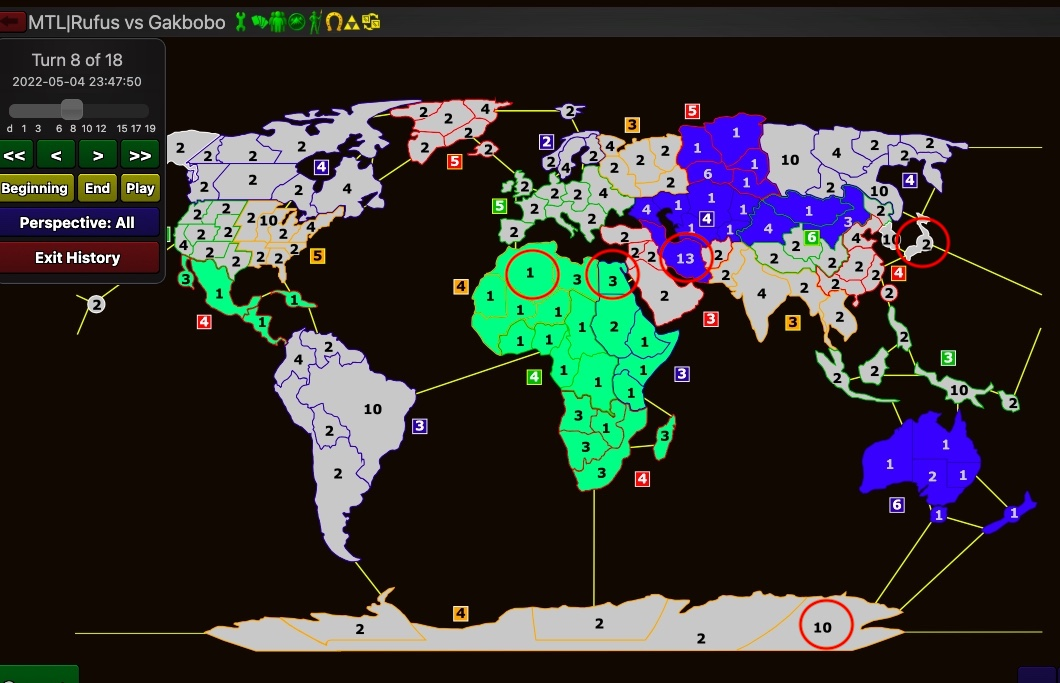
\includegraphics[width=0.9\textwidth]{Images/rand_gak_rufus.jpg}
  \caption{Position end of T8 Gak vs Rufus}
  \label{gak_rufus}
\end{figure}
    \begin{enumerate}
        \item As Rufus, the game is all about a) securing Iran, b) breaking Africa and c) potentially securing Japan. With WC 26, with EC 30 income, that's more than what Africa can offer. Breaking the wasteland in Antarctica is under no circumstance the way to go, too many armies for a single border and Gak has leftovers in SAf. The issue with Iran stack to break Egypt is Gak can blockade Egypt and Gak can also pivot to NA, flank Japan, and enter Asia
        \item As Gak, it is a question of reaching Rufus income before he reaches yours.
    \end{enumerate}
    \item Try to evaluate yourself the position and what's the correct approach. Lengthy WR games can be broken down to utilizing all the tempo advantage you can get. Rufus breaks Af 1 turn before Gak breaks Asia (and only Caucasus), as he misses the Pakistan line. There are a lot of different and potentially better approaches (not to say the players misplayed as they real-timed it), but consider Gak's position with 10 less armies between Egypt/Ant and having Japan. T12 you have an army disadvantage in Egypt potentially, a free gamble in Aus and a pathway from Japan. At the end of the day both here and in MME, and MALD and every modified earth clone, in Asia vs Africa positions where both players break each other roughly on the same turn, Asia wins. The reason is the border alignment, quite simply. If you break Algeria within 2 turns you have broken 3/4 Africa bonuses. If you break Iran, within 3 turns you get to break WC, CR and within 5 turns EC and ER. 
\end{itemize}

The concept of pivoting to safer income applies less often in Randomized ME than other WR templates due to most games finishing in the early game. Take for example \href{https://www.warzone.com/MultiPlayer?GameID=38698474}{this game} from T5 onwards. As Octane, you are ahead, more income, more expansion zones, no need to take a risk or waste armies in neutrals moving towards the opponent, as they have nowhere to expand but towards Aus and Greenland. SEA, WC, Canada and WR are free bonuses to pivot to. Even after T9, where Rufus has found a way to comeback and muddy the waters, you need to play for the winning idea. No matter what Rufus is not allowed to break Greenland and Canada, that's 16 income by itself. As Octane if you break Algeria and move onwards, Rufus drops to 11 income in 2 turns and the game is won as long as we build a stack in Aus/Indo. Simplify position towards a line that nets you a win.